\begin{frame}
    \frametitle{Modeling Decentralized POMDP}
    \begin{block}{Example: Dec-POMDP}
        \begin{figure}
            \centering
            \documentclass{standalone}

\usepackage{tikz-qtree}
\usepackage{circuitikz}
\usetikzlibrary{positioning,arrows}
\usepackage{rotating}
\newcommand{\random}[1]{\rotatebox[origin=c]{180}{$\mathsf{R}$}^{#1}} % randomized quantifier

\usetikzlibrary{automata}
\begin{document}
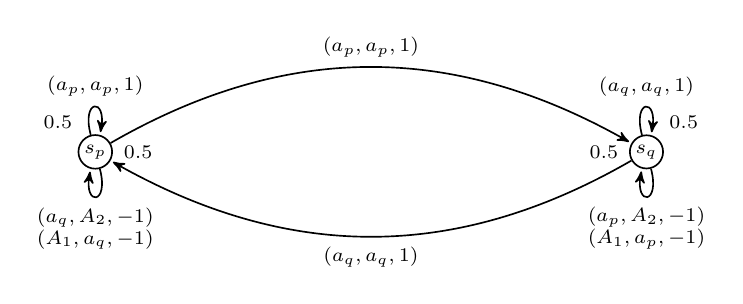
\begin{tikzpicture}[->,>=stealth',shorten >=1pt,auto,node distance=7cm,semithick]
    \tikzstyle{every node}=[font=\scriptsize]
    \node[state,inner sep=1pt,minimum size=0pt] (P) {$s_p$};
    \node[state,inner sep=1pt,minimum size=0pt] (Q) [right of=P] {$s_q$};
    \node[above left = 0.01 cm of P] {$0.5$};
    \node[right = 0.01 cm of P] {$0.5$};
    \node[above right = 0.01 cm of Q] {$0.5$};
    \node[left = 0.01 cm of Q] {$0.5$};

    \path
    (P) edge [bend left] node {$(a_p,a_p,1)$} (Q)
    edge [loop above] node {$(a_p,a_p,1)$} (P)
    edge [loop below] node[align=left] {$(a_q,A_2,-1)$\\$(A_1,a_q,-1)$} (P)
    (Q) edge [bend left] node {$(a_q,a_q,1)$} (P)
    edge [loop above] node {$(a_q,a_q,1)$} (Q)
    edge [loop below] node[align=left] {$(a_p,A_2,-1)$\\$(A_1,a_p,-1)$} (Q);
\end{tikzpicture}
\end{document}
        \end{figure}
        $\mathcal{M}=(\{1,2\},\{s_p,s_q\},\{a_p,a_q\},T,\rho,\{o_p,o_q\},\Omega,\Delta_0,h)$
        \begin{itemize}
            \item $T(s_p,a_p,a_p,s_p)=T(s_p,a_p,a_p,s_q)=0.5$
            \item $\rho(s_p,a_p,a_p)=1;\rho(s_p,a_q,A_2)=\rho(s_p,A_1,a_q)=-1$
            \item $\Omega(s_p,o_p)=\spb{o_p|s_p}$
        \end{itemize}
    \end{block}
\end{frame}

\begin{frame}
    \frametitle{Modeling Decentralized POMDP}
    \begin{itemize}
        \item Optimal \emph{joint policy} to maximize the expected total reward
              \begin{itemize}
                  \item An agent can only base its actions on \alert{its own observations}
                  \item NEXPTIME-completeness~\cite{Bernstein2002}
              \end{itemize}
              \pause
        \item Policy selection for an individual agent~\cite{Salmon2020}
              \begin{itemize}
                  \item Agent~$1$: $\exists x_a^{1,0},\random{} x_o^{1,0},\exists x_a^{1,1},\random{} x_o^{1,1},\exists x_a^{1,2},\ldots$
                  \item Agent~$2$: $\exists x_a^{2,0},\random{} x_o^{2,0},\exists x_a^{2,1},\random{} x_o^{2,1},\exists x_a^{2,2},\ldots$
                  \item A linearly ordered prefix for all agents?
              \end{itemize}
              \pause
        \item Explicitly specify dependency sets in DSSAT
              \begin{itemize}
                  \item $\random{}x_o^{1,0},\random{}x_o^{2,0},\random{}x_o^{1,1},\random{}x_o^{2,1},\exists x_a^{1,0},\exists x_a^{1,1}(\{x_o^{1,0}\}),\exists x_a^{1,2}(\{x_o^{1,0},x_o^{1,1}\}),\ldots$
              \end{itemize}
    \end{itemize}
\end{frame}